\documentclass[12pt]{article}
\usepackage[utf8]{inputenc}
\usepackage[brazil]{babel}
\usepackage{graphicx}
\usepackage{listings}
\usepackage{xcolor}
\usepackage{amsmath}
\usepackage{geometry}
\usepackage{float}
\usepackage{subcaption}
\lstset{showstringspaces=false}
\geometry{a4paper, margin=2.5cm}

% Configuração para códigos Matlab
\lstset{
    language=Matlab,
    basicstyle=\ttfamily\small,
    keywordstyle=\color{blue},
    stringstyle=\color{red},
    commentstyle=\color{green!60!black},
    numbers=left,
    numberstyle=\tiny,
    stepnumber=1,
    frame=single,
    breaklines=true,
    extendedchars=true,
    literate={á}{{\'a}}1 {ã}{{\~a}}1 {õ}{{\~o}}1 {é}{{\'e}}1 {í}{{\'i}}1 {ó}{{\'o}}1 {ú}{{\'u}}1 {ç}{{\c{c}}}1
}

\title{Relatório: Prática 2 - Transformada Discreta de Fourier e Resposta em Frequência \\ \large Análise de Sistemas Lineares - UTFPR}
\author{Leonardo Pereira Shibata \\ Sergio Roncato Maccari}
\date{Abril de 2026}

\begin{document}

\begin{titlepage}
    \begin{center}
        \Large \textbf{UNIVERSIDADE TECNOLÓGICA FEDERAL DO PARANÁ} \\
        \Large \textbf{CURSO DE ENGENHARIA DE COMPUTAÇÃO} \\
        \large ELEQ30 - Análise de Sistemas Lineares \\
        \large Professor César Janeczko \\
        \vspace{5cm}
        \huge \textbf{Relatório: Prática 2} \\
        \large \textbf{Transformada Discreta de Fourier e Resposta em Frequência} \\
        \vspace{1.5cm}
        \Large \textbf{Disciplina: Análise de Sistemas Lineares} \\
        \vspace{4cm}
        \Large Leonardo Pereira Shibata \\
        \Large Sergio Roncato Maccari \\
        \vfill
        \Large Curitiba, Abril de 2026
    \end{center}
\end{titlepage}

\section{Transformada Discreta de Fourier - DFT}

\subsection{Implementação da função DFT (algoritmo em Basic)}

A função abaixo segue fielmente o algoritmo em Basic do anexo, percorrendo todas as amostras de saída $K$ e correlacionando o sinal de entrada com cossenos e senos.
A saída é montada como $Y = REX + \sqrt{-1}\cdot IMX$, conforme solicitado.

\begin{lstlisting}
function [Y] = DFT(XX)
    NX = length(XX);
    REX(floor(NX/2) + 1) = 0;
    IMX(floor(NX/2) + 1) = 0;
    for K = 1:(floor(NX/2) + 1)
        for I = 1:NX
            REX(K) = REX(K) + XX(I) * cos(2 * pi * (K-1) * (I-1) / NX);
            IMX(K) = IMX(K) - XX(I) * sin(2 * pi * (K-1) * (I-1) / NX);
        end
        Y = REX + sqrt(-1) * IMX;
    end
end
\end{lstlisting}

\subsection{Elaboração do sinal (janela de 1000 amostras)}

$$x(n) = \cos(\pi(n-1)/50) + \cos(\pi(n-1)/5{,}5) + \sin(\pi(n-1)/5)$$

\textbf{Plot do sinal elaborado no tempo discreto $n$ (n = número de amostras):}

\begin{lstlisting}
fs = 1000;  % Frequencia de amostragem (Hz)
N  = 1000;  % Tamanho da janela
n  = 1:N;   % Indice da amostra (1 a 1000)

x = cos(pi*(n-1)/50) + cos(pi*(n-1)/5.5) + sin(pi*(n-1)/5);

figure('Name', '1.b) - Elaboração do sinal x(n)');
plot(x); title('sinal com 3 frequencia');
\end{lstlisting}

\begin{figure}[H]
    \centering
    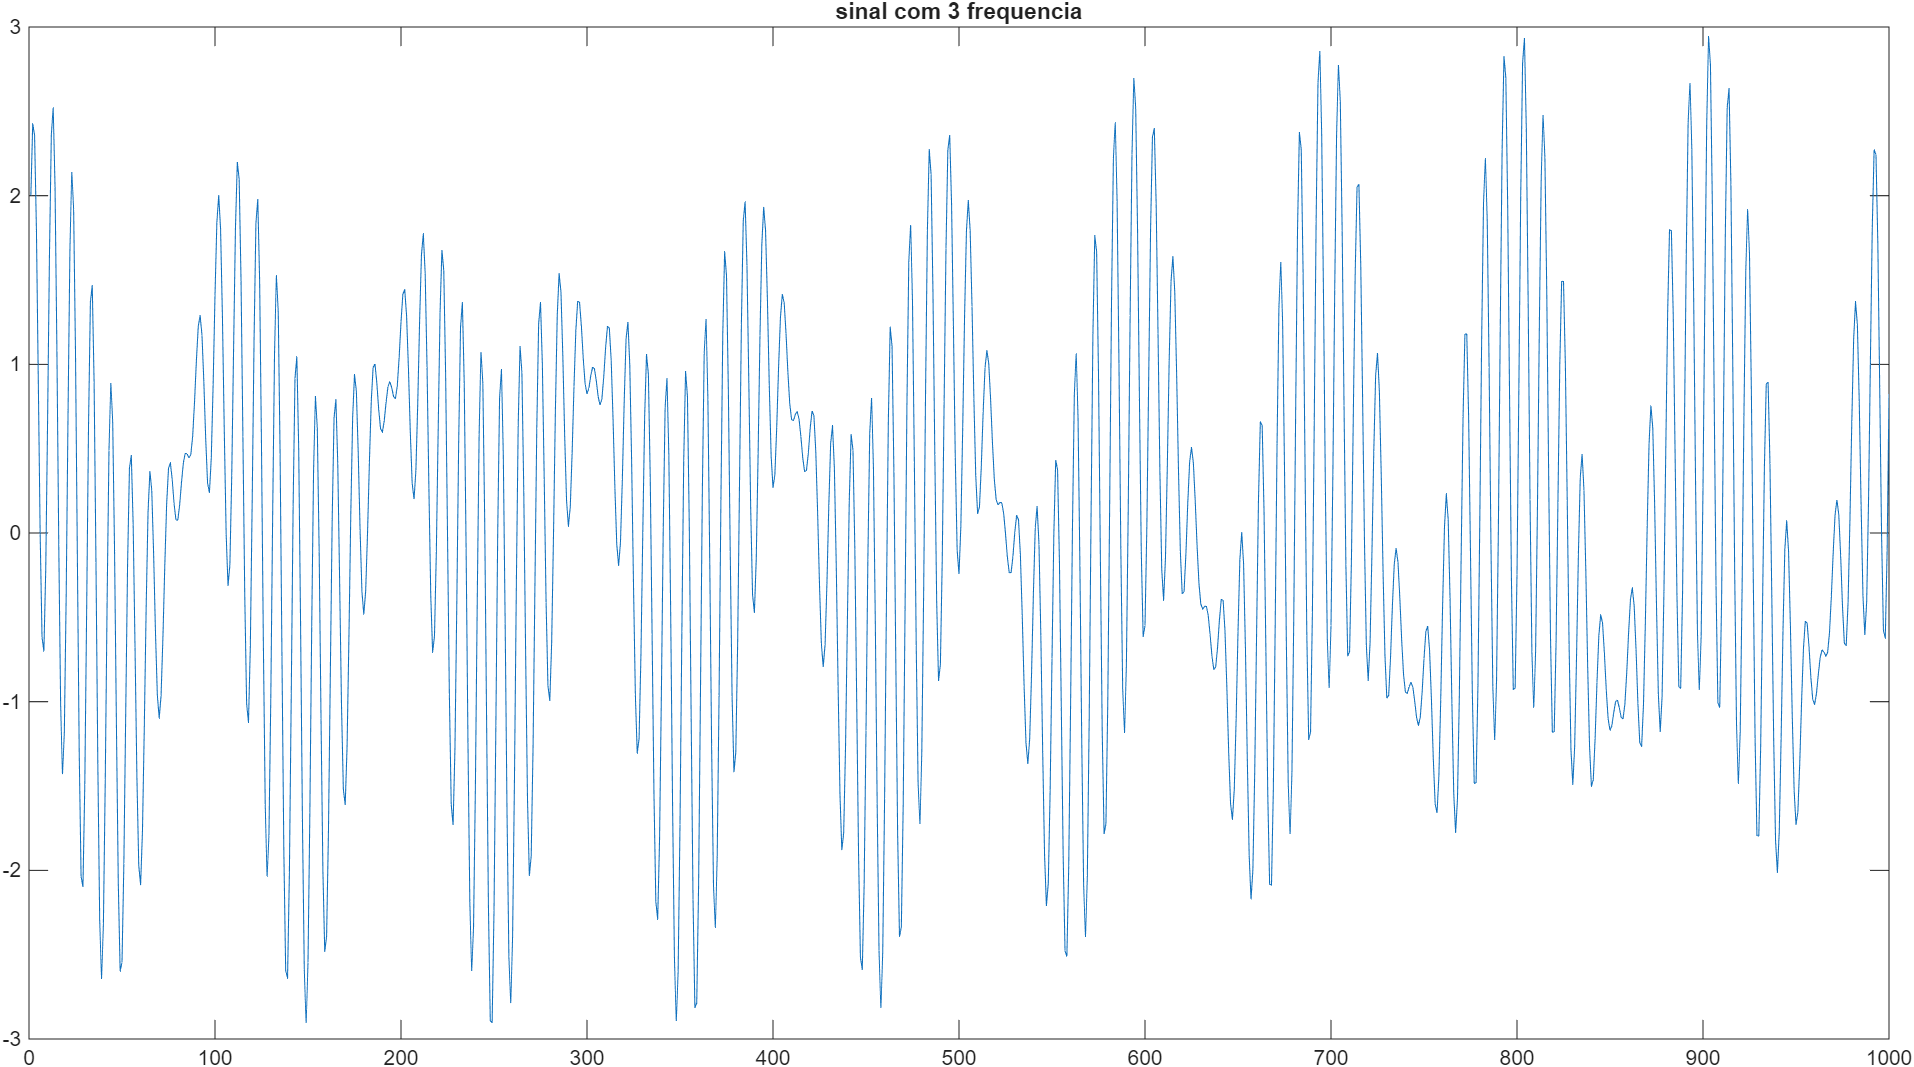
\includegraphics[width=0.9\textwidth]{imgs/1_b_sinal_3_frequencia.png}
    \caption{Sinal $x(n)$ com 1000 amostras no tempo discreto, composto pela soma de três componentes harmônicas.}
\end{figure}

\subsection{Componentes de frequência do sinal $x(n)$}

Comparando cada argumento com a forma genérica $\dfrac{2\pi f\, n}{f_s}$, com $f_s = 1000\,\text{Hz}$, e usando a relação $f = \dfrac{\omega}{2\pi}\cdot f_s$:

\textbf{1º Cosseno:} $\cos\left(\dfrac{\pi(n-1)}{50}\right)$
$$\omega_1 = \frac{\pi}{50} \;\Rightarrow\; f_1 = \frac{\pi/50}{2\pi}\cdot 1000 = \frac{1000}{100} = 10\,\text{Hz}$$

\textbf{2º Cosseno:} $\cos\left(\dfrac{\pi(n-1)}{5{,}5}\right)$
$$\omega_2 = \frac{\pi}{5{,}5} \;\Rightarrow\; f_2 = \frac{\pi/5{,}5}{2\pi}\cdot 1000 = \frac{1000}{11} \approx 90{,}91\,\text{Hz}$$

\textbf{Seno:} $\sin\left(\dfrac{\pi(n-1)}{5}\right)$
$$\omega_3 = \frac{\pi}{5} \;\Rightarrow\; f_3 = \frac{\pi/5}{2\pi}\cdot 1000 = \frac{1000}{10} = 100\,\text{Hz}$$

Portanto, as componentes de frequência presentes no sinal são, aproximadamente,
\textbf{10 Hz}, \textbf{90,91 Hz} e \textbf{100 Hz}.

\subsection{Cálculo da DFT pelo algoritmo próprio e pela FFT do MATLAB}

Compare-se os resultados e os tempos de execução:

\begin{lstlisting}
disp('Calculando DFT elaborada...');
tic(); dftx = DFT(x); tempo_dft = toc();
fprintf('Tempo DFT: %f segundos\n', tempo_dft);

disp('Calculando FFT nativa...');
tic(); fftx = fft(x); tempo_fft = toc();
fprintf('Tempo FFT: %f segundos\n', tempo_fft);
\end{lstlisting}

Os resultados numéricos da DFT implementada e da \texttt{fft()} nativa são equivalentes
(diferenças apenas devido a arredondamento de ponto flutuante). Já em relação ao tempo
de execução, a função \texttt{DFT} possui complexidade $O(N^2)$ (dois laços aninhados de
$N$ iterações), enquanto a \texttt{fft} do MATLAB utiliza o algoritmo \textit{Fast Fourier
Transform}, com complexidade $O(N\log N)$. Para $N = 1000$ amostras, observa-se uma
diferença de várias ordens de grandeza no tempo de processamento, sendo a \texttt{fft}
muito mais rápida. Cabe lembrar que o tempo medido pelo \texttt{tic/toc} sofre influência
de outros processos em execução paralela no sistema operacional.

\subsection{Gráficos abs / real / imag da DFT}

\begin{lstlisting}
figure('Name', '1.e) - Análise do Sinal x(n)');
subplot(3,1,1); plot(abs(dftx));  title('abs DFT');
subplot(3,1,2); plot(real(dftx)); title('real DFT');
subplot(3,1,3); plot(imag(dftx)); title('imag DFT');
\end{lstlisting}

\begin{figure}[H]
    \centering
    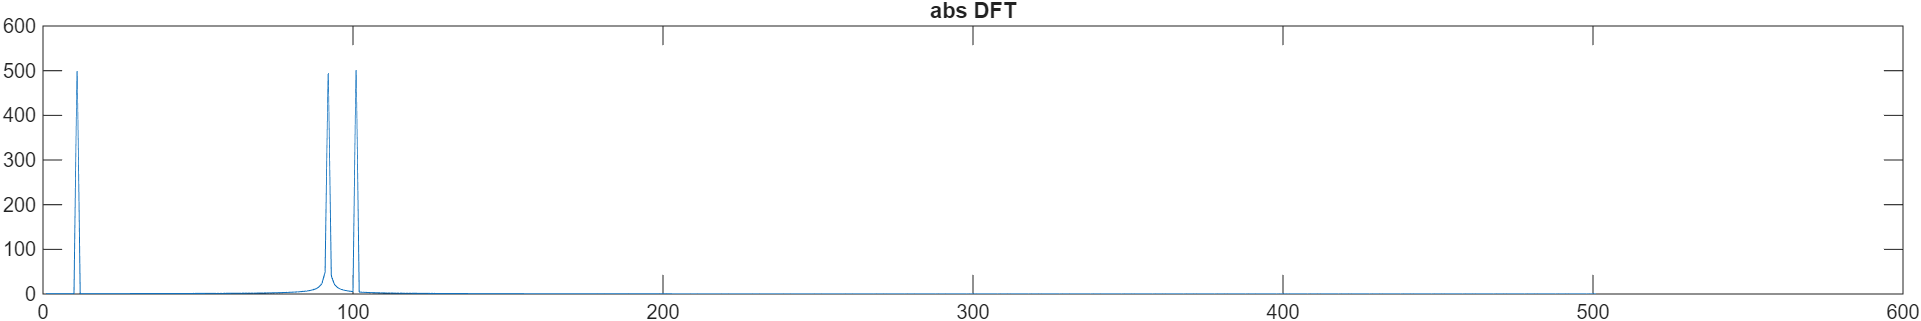
\includegraphics[width=0.85\textwidth]{imgs/abs_DFT.png}
    \caption{Módulo da DFT de $x(n)$ — $|\mathrm{DFT}(x)|$. Observam-se três picos correspondentes às componentes de 10\,Hz, 90,91\,Hz e 100\,Hz.}
\end{figure}

\begin{figure}[H]
    \centering
    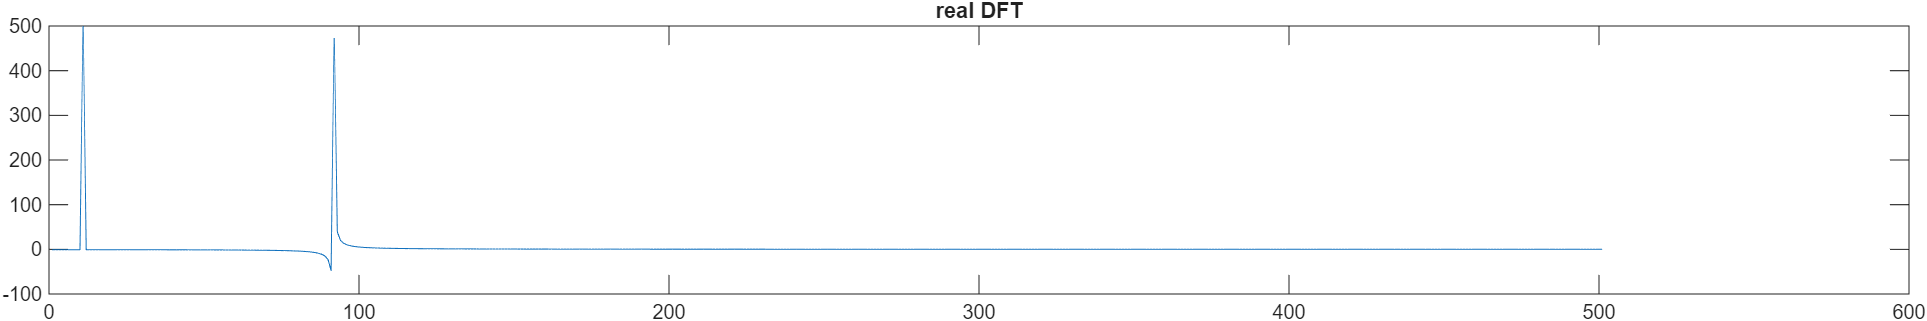
\includegraphics[width=0.85\textwidth]{imgs/real_DFT.png}
    \caption{Parte real da DFT de $x(n)$ — $\mathrm{Re}\{\mathrm{DFT}(x)\}$. Os cossenos com frequência de raia inteira (10\,Hz) projetam-se exclusivamente sobre a base cosseno.}
\end{figure}

\begin{figure}[H]
    \centering
    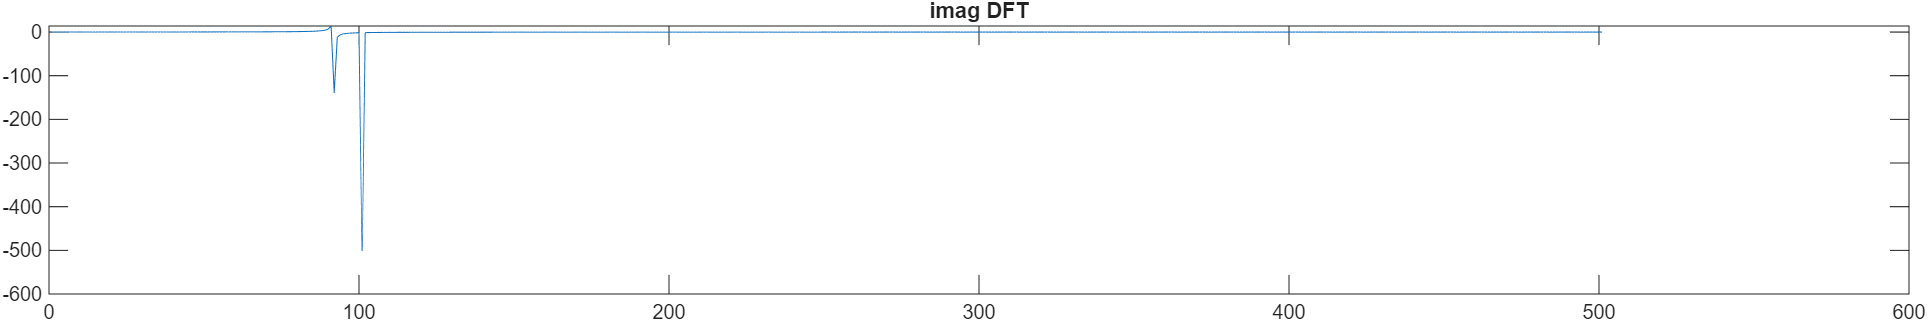
\includegraphics[width=0.85\textwidth]{imgs/imag_DFT.png}
    \caption{Parte imaginária da DFT de $x(n)$ — $\mathrm{Im}\{\mathrm{DFT}(x)\}$. O seno em 100\,Hz aparece como imaginário puro (negativo).}
\end{figure}

\textbf{Explicação:} a DFT é, essencialmente, uma correlação do sinal de entrada com
cossenos (parte real) e senos (parte imaginária, com sinal negativo). Quando uma componente
do sinal cai \textit{exatamente} sobre uma raia inteira da DFT (ou seja, completa um número
inteiro de períodos dentro da janela de $N$ amostras), a sua energia se concentra em uma
única amostra do espectro:

\begin{itemize}
    \item $\cos(\pi(n-1)/50)$ tem $f_1 = 10$ Hz e cai exatamente em $k = 10$ (pois
    $k = f_1\cdot N/f_s = 10\cdot 1000/1000 = 10$). Como cosseno é uma função par,
    correlaciona perfeitamente com a base cosseno e zero com a base seno, resultando em
    \textbf{parte real pura}.

    \item $\sin(\pi(n-1)/5)$ tem $f_3 = 100$ Hz e cai exatamente em $k = 100$.
    Como seno é uma função ímpar, correlaciona perfeitamente com a base seno e zero com
    a base cosseno, resultando em \textbf{parte imaginária pura} (negativa, devido ao
    sinal $-\sin$ na definição da DFT).

    \item $\cos(\pi(n-1)/5{,}5)$ tem $f_2 \approx 90{,}91$ Hz, cuja raia ideal seria
    $k \approx 90{,}91$ — \textbf{não inteira}. Como a DFT só calcula amostras em valores
    inteiros de $k$, ocorre o fenômeno de \textit{spectral leakage} (vazamento espectral):
    a energia se espalha pelas raias vizinhas e aparece tanto na parte real quanto na
    imaginária do espectro.
\end{itemize}

\clearpage

\section{Aumentar a Resolução em Frequência}

\subsection{Refazer o sinal com 150 pontos e aplicar zero-padding}

Refaça o sinal $x(n)$ (chamando-o de $x_1$) com apenas 150 pontos
(mantendo $f_s = 1000\,\text{Hz}$). Plot $x_1$ no tempo e na frequência. Em seguida,
preencha $x_1$ com zeros até 1000 pontos e refaça as plotagens. Conclua sobre o efeito
do preenchimento com zeros.

\begin{lstlisting}
% Sinal reduzido para 150 pontos
N1 = 150;
n1 = 1:N1;
x1 = cos(pi*(n1-1)/50) + cos(pi*(n1-1)/5.5) + sin(pi*(n1-1)/5);

figure('Name', '2 - Aumentar a resolução em frequência');

subplot(2,2,1); plot(x1);                title('x1 (150 pontos) no Tempo');
subplot(2,2,2); plot(abs(DFT(x1)),'.-'); title('DFT x1 (150 pontos)');

% Preenchendo com zeros até 1000 pontos
x1_pz = [x1, zeros(1, N - N1)];

subplot(2,2,3); plot(x1_pz);                title('x1 com zeros (1000 pt) no Tempo');
subplot(2,2,4); plot(abs(DFT(x1_pz)),'.-'); title('DFT x1 com zeros');
\end{lstlisting}

\begin{figure}[H]
    \centering
    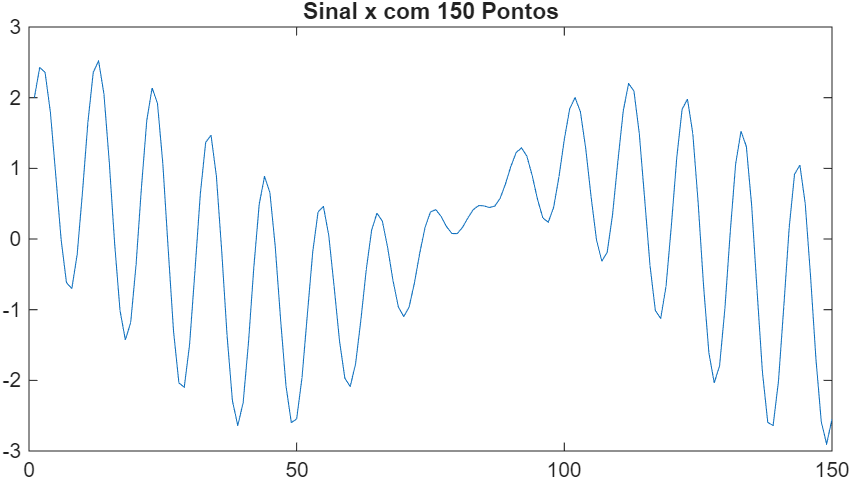
\includegraphics[width=0.78\textwidth]{imgs/sinal_x_com_150_pontos.png}
    \caption{Sinal $x_1$ com 150 pontos no tempo discreto.}
\end{figure}

\begin{figure}[H]
    \centering
    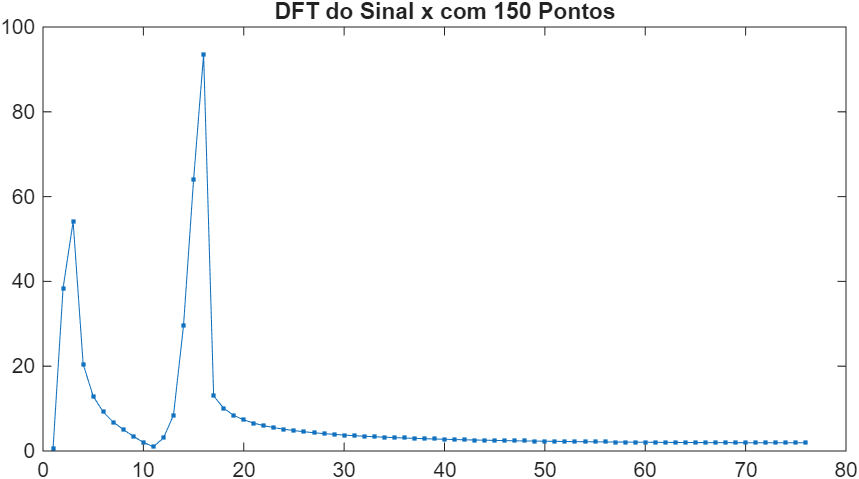
\includegraphics[width=0.78\textwidth]{imgs/DFT_do_sinal_x_com_150_pontos.png}
    \caption{Módulo da DFT do sinal $x_1$ com 150 pontos. Os picos das três componentes aparecem misturados, sem boa separação entre 90,91\,Hz e 100\,Hz.}
\end{figure}

\begin{figure}[H]
    \centering
    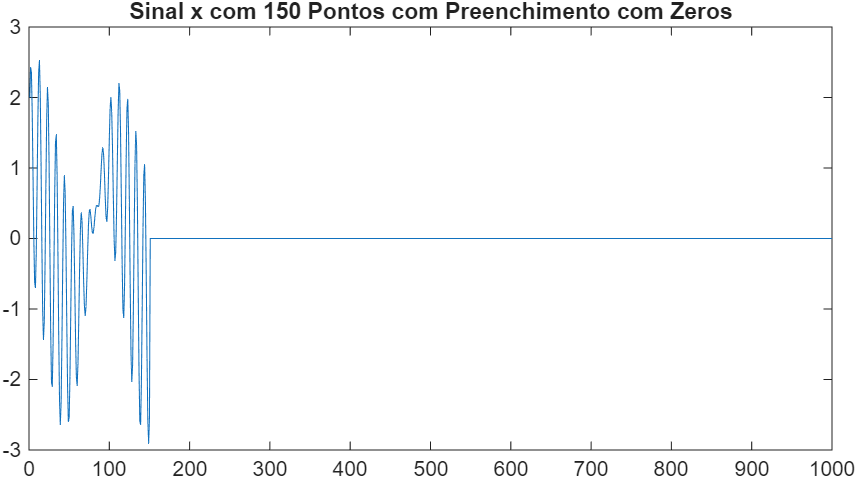
\includegraphics[width=0.78\textwidth]{imgs/sinal_x_com_150_pontos_com_preenchimento_com_zeros.png}
    \caption{Sinal $x_1$ preenchido com zeros até 1000 pontos no tempo discreto (\textit{zero-padding}).}
\end{figure}

\begin{figure}[H]
    \centering
    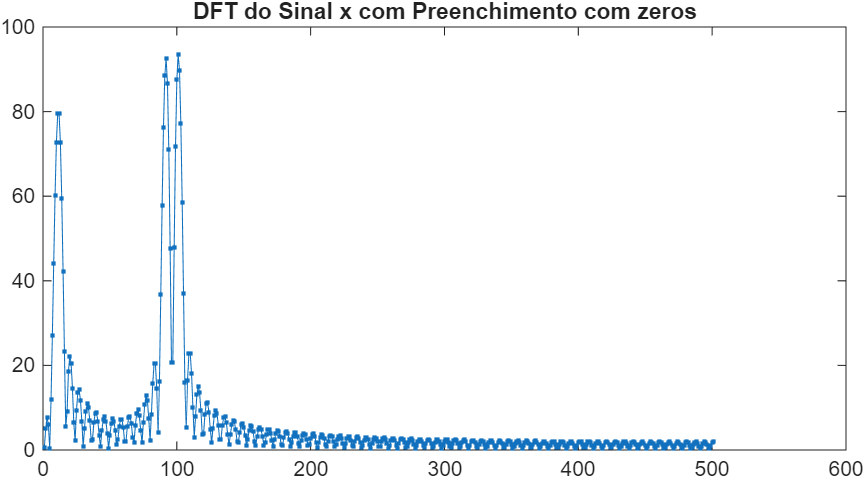
\includegraphics[width=0.78\textwidth]{imgs/DFT_do_sinal_x_com_preenchimento_com_zeros.png}
    \caption{Módulo da DFT do sinal $x_1$ preenchido com zeros até 1000 pontos. O espectro fica visivelmente mais denso e suave (interpolado), embora a resolução real em frequência continue limitada pelos 150 pontos originais.}
\end{figure}

\textbf{Conclusão:} o preenchimento com zeros (\textit{zero-padding}) \textbf{não aumenta
a resolução real em frequência} do sinal. A resolução em frequência verdadeira é
determinada pelo tempo total de observação do sinal,
$\Delta f = f_s/N_{\text{real}}$, onde $N_{\text{real}}$ é o número de amostras
\textit{efetivamente medidas}. Com 150 pontos, $\Delta f \approx 6{,}67\,\text{Hz}$;
ao adicionar zeros, esse limite físico não muda.

O que o \textit{zero-padding} faz é \textbf{interpolar} o espectro: o espectro contínuo
subjacente passa a ser amostrado em um número maior de pontos, tornando o gráfico mais
denso e suave (mais fácil de visualizar e localizar visualmente os picos). Porém,
nenhuma informação nova é criada — picos próximos que estavam misturados continuam
misturados, apenas com aparência mais ``contínua''.

\clearpage

\section{Resposta em Frequência}

\subsection{Resposta em frequência (ganho) do sinal \texttt{fpf.mat}}

Geram-se o gráfico da função no tempo (resposta ao impulso, $h_{FPF}$) e do sinal obtido
como resultado da DFT (Curva de Ganho, \texttt{abs(DFT(fpf))}).

\begin{lstlisting}
load('fpf.mat');

figure('Name', '3 - Resposta em Frequência');

subplot(2,2,1); plot(fpf, '.-');           title('Resposta ao Impulso Original (hFPF)');
subplot(2,2,2); plot(abs(DFT(fpf)), '.-'); title('Ganho Original');
\end{lstlisting}

\begin{figure}[H]
    \centering
    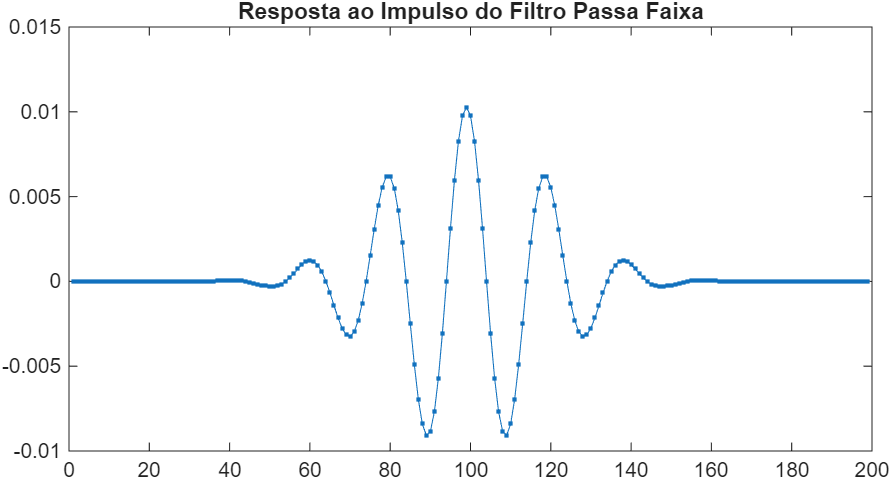
\includegraphics[width=0.85\textwidth]{resposta_impulso_filtro_passa_faixa.png}
    \caption{Resposta ao impulso $h_{FPF}$ do filtro passa-faixa original (199 amostras).}
\end{figure}

\begin{figure}[H]
    \centering
    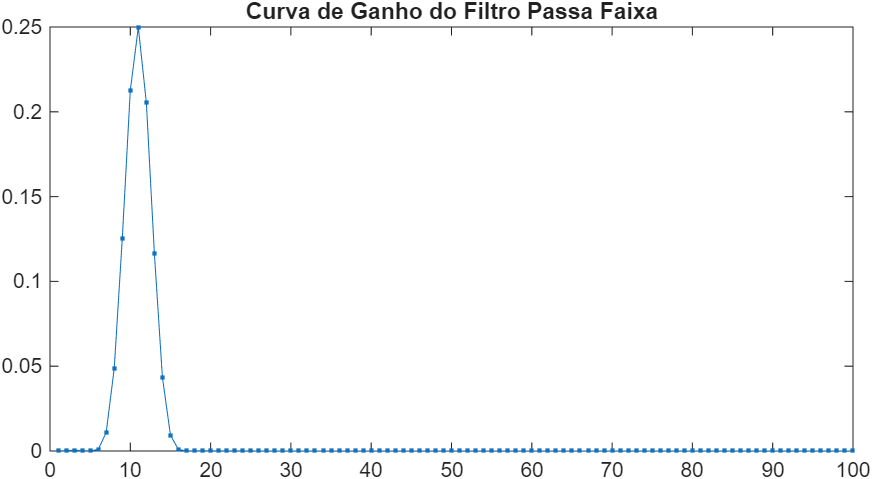
\includegraphics[width=0.85\textwidth]{curva_ganho_filtro_passa_faixa.png}
    \caption{Curva de ganho do filtro passa-faixa original — $|\mathrm{DFT}(fpf)|$. Observa-se um lobo central centrado na frequência de passagem do filtro.}
\end{figure}

A resposta ao impulso $h_{FPF}$ apresenta um número limitado de amostras (199 pontos),
e a curva de ganho obtida pela DFT mostra o comportamento típico de um filtro
passa-faixa, amostrado de forma esparsa devido ao número reduzido de pontos.

\subsection{Preenchimento de \texttt{fpf} com zeros até 1000 pontos}

Repita as plotagens do item anterior com o novo sinal preenchido. Verifique que a escala
de frequência mudou, mas sempre proporcional à frequência de amostragem.

\begin{lstlisting}
fpf_zp = [fpf(:)', zeros(1, 1000 - length(fpf))];

subplot(2,2,3); plot(fpf_zp, '.-');           title('hFPF com preenchimento com zeros');
subplot(2,2,4); plot(abs(DFT(fpf_zp)), '.-'); title('Ganho com preenchimento com zeros');
\end{lstlisting}

\begin{figure}[H]
    \centering
    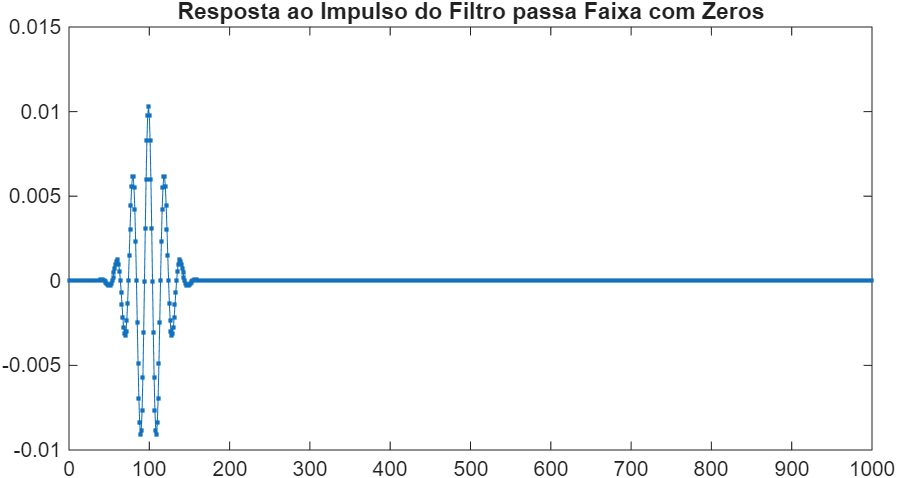
\includegraphics[width=0.85\textwidth]{resposta_impulso_filtro_passa_faixa_zeros.png}
    \caption{Resposta ao impulso $h_{FPF}$ preenchida com zeros até 1000 amostras. Os coeficientes não-nulos permanecem nas primeiras 199 posições, e o restante é zero.}
\end{figure}

\begin{figure}[H]
    \centering
    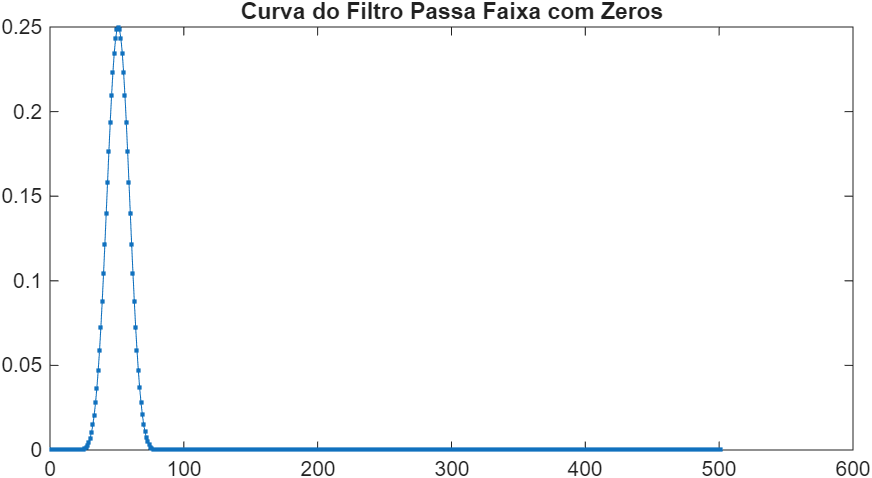
\includegraphics[width=0.85\textwidth]{curva_filtro_passa_faixa_zeros.png}
    \caption{Curva de ganho do filtro passa-faixa após \textit{zero-padding} para 1000 pontos. O lobo central aparece muito mais bem amostrado (densidade espectral interpolada).}
\end{figure}

\textbf{Conclusões:} o eixo horizontal (índice $k$) muda de escala conforme o número de
pontos da DFT. No sinal original, o índice $k = 199$ corresponde à frequência de
amostragem $f_s$; com o sinal preenchido até 1000 pontos, é $k = 1000$ que corresponde a
$f_s$. Em ambos os casos, a frequência associada a cada raia é $f_k = k\cdot f_s/N$, ou seja,
\textbf{sempre proporcional à frequência de amostragem}.

A curva de ganho \textit{em si} é a mesma função: o \textit{zero-padding} apenas a
amostrou em mais pontos, fornecendo uma visualização mais detalhada (interpolada) da
resposta em frequência do filtro, sem alterar a sua característica real. Esta conclusão
é coerente com a obtida na Seção 2: o preenchimento com zeros melhora apenas a
\textbf{resolução de visualização}, e não a resolução física em frequência.

\section{Conclusão Final}

A prática permitiu compreender, na prática, a Transformada Discreta de Fourier e a
resposta em frequência de sinais discretos. A implementação manual da DFT, embora
didática e fiel ao algoritmo clássico, mostrou-se computacionalmente custosa
($O(N^2)$) quando comparada à \texttt{fft()} nativa do MATLAB, que utiliza o algoritmo
FFT com complexidade $O(N\log N)$ — justificando o seu uso em aplicações reais.

A análise dos componentes do espectro (parte real, imaginária e módulo) evidenciou
a relação direta entre simetria do sinal no tempo (par/ímpar) e a sua projeção sobre
as bases cosseno/seno da DFT, bem como o fenômeno de \textit{spectral leakage} quando
uma componente não cai exatamente sobre uma raia inteira da DFT.

Por fim, ficou claro que o preenchimento com zeros (\textit{zero-padding}) não aumenta
a resolução real em frequência — esta depende exclusivamente do tempo total de observação
do sinal — mas sim a \textbf{densidade de amostragem do espectro}, atuando como uma
interpolação que facilita a visualização e a localização dos picos. Esta conclusão se
verificou tanto no sinal $x_1$ (Seção 2) quanto no filtro \texttt{fpf} (Seção 3),
reforçando que a relação $\Delta f = f_s/N$ governa a resolução em frequência da DFT.

\end{document}
